% ============================================================================
% P4 — Pareto-Guided Monte Carlo Tree Search for Antimalarial Design
% Target: Journal of Cheminformatics (BMC)
% Strategy: honest ranking (Random ≥ MCTS on mean reward);
%           MCTS value = multi-objective Pareto exploration
% ============================================================================
\documentclass[10pt,a4paper]{article}

\usepackage[margin=2.2cm]{geometry}
\usepackage[T1]{fontenc}
\usepackage[utf8]{inputenc}
\usepackage{lmodern}
\usepackage{amsmath,amssymb}
\usepackage{booktabs}
\usepackage{graphicx}
\graphicspath{{Graphics/}}
\usepackage{siunitx}
\usepackage{microtype}
\usepackage{enumitem}
\usepackage{xcolor}
\usepackage[colorlinks=true,linkcolor=blue,citecolor=blue,urlcolor=blue]{hyperref}
\usepackage{xr-hyper}
\externaldocument[SM-]{P4_Pareto_MCTS_JoC_SM}
\usepackage[nameinlink,noabbrev]{cleveref}
\usepackage{natbib}

\sisetup{
  detect-all           = true,
  group-minimum-digits = 4,
  range-phrase         = {--},
  range-units          = single,
}

\title{\textbf{Pareto-guided Monte Carlo tree search reveals multi-objective trade-offs\\ in antimalarial generation}}

\author{%
  \begin{tabular}{c}
  Myke Vital Sao Temgoua$^{1}$, Jean-Pierre Tchapet Njafa$^{1}$, Serge Guy Nana Engo$^{1}$\\
  Penabei Samafou$^{2}$, Wilfred Fon Mbacham$^{3}$\\[0.2em]
  \small Corresponding author: \texttt{myke-vital.sao@facsciences-uy1.cm}
  \end{tabular}
}

\date{}

\begin{document}
\maketitle

\begin{center}
\begin{minipage}{0.92\textwidth}
\small\raggedright
$^{1}$Department of Physics, Faculty of Science, University of Yaound\'{e} I, P.O.\ Box 812, Yaound\'{e}, Cameroon\\
$^{2}$Department of Medical Imaging and Radiation Sciences, Universit\'{e} de Sherbrooke, Sherbrooke, QC, Canada\\
$^{3}$Department of Biochemistry, Faculty of Science, University of Yaound\'{e} I, P.O.\ Box 812, Yaound\'{e}, Cameroon
\end{minipage}
\end{center}

\begin{abstract}
\noindent
Scalar rewards can conceal trade-offs in de novo molecular design. We therefore separate scalar performance from multi-objective coverage. We present a Pareto-guided Monte Carlo tree search (MCTS) framework that records a pre-activity candidate front across multi-parameter optimisation (MPO), synthetic Bayesian accessibility (SYBA), an RRS-informed chemotype-similarity proxy and a PNS-informed Tartarus docking proxy, using a scaffold-aware fragment policy informed by ChEMBL27 frequencies and Tanimoto compatibility. In the deposited historical run, SYBA returned a constant zero fallback during search and was therefore not an informative search-time objective; it was recomputed transparently before the final front was re-derived. In the v12 scalar benchmark, conducted with \num{20} independent seeds and a public-activity proximity term, random search had the highest mean reward (\num{0.6724} $\pm$ \num{0.0056}), followed by MCTS (\num{0.6649} $\pm$ \num{0.0068}), the genetic algorithm (\num{0.6453} $\pm$ \num{0.0124}) and greedy search (\num{0.4278} $\pm$ \num{0.0000}). MCTS was below random (paired $t_{19}=\num{-4.97}$, $p=\num{0.000085}$, mean $\Delta=\num{-0.0075}$, 95\% CI $[\num{-0.0107},\,\num{-0.0043}]$) but above the genetic algorithm ($t_{19}=\num{6.95}$, $p<\num{0.0001}$). In the separate historical pre-activity analysis, MCTS yielded four mutually non-dominated solutions after the documented post-hoc SYBA re-derivation (hypervolume \num{1.2366}), including a high-MPO/low-SYBA extreme discarded by fixed-weight scalar aggregation. The results position MCTS as a transparent multi-objective explorer, not as a universally superior scalar optimiser; the RRS/PNS-informed dimensions are integrated proxies whose biological validation remains future work.
\end{abstract}

\textbf{Scientific Contribution:} We introduce a Pareto-guided MCTS framework for de novo antimalarial design and evaluate it through two explicitly separated analyses. The deposited pre-activity search records a vector schema comprising MPO, SYBA, an RRS-informed chemotype proxy and a PNS-informed Tartarus docking proxy. MPO and the RRS/PNS-informed signals were available during the historical search; SYBA was constant at zero in the search-time records and was used only in the documented post-hoc front re-derivation. The v12 scalar benchmark adds public-activity proximity but disables the two domain proxies, allowing a fair scalar comparison with random, greedy and genetic baselines. MCTS is below random on scalar reward (mean $\Delta = -\num{0.0075}$, $p = \num{0.000085}$; 95\% CI $[\num{-0.0107},\,\num{-0.0043}]$), yet yields an audited post-hoc front spanning the potency--accessibility trade-off. The contribution is therefore transparent objective-space exploration, not scalar superiority or direct biological validation.

\noindent\textbf{Keywords:} de novo design; Monte Carlo tree search; Pareto optimisation; antimalarial; multi-objective; synthetic accessibility; resistance resilience

% ============================================================================
\section{Introduction}
% ============================================================================

Malaria remains one of the leading infectious causes of death in sub-Saharan Africa---an estimated \num{247} million cases and \num{619000} deaths in 2023 \citep{WHO2024MalariaReport}---and control is increasingly threatened by artemisinin-resistant \emph{Plasmodium falciparum} strains in Southeast Asia and Africa \citep{Ariey2014,Ashley2018}. Mitigating antimalarial drug resistance therefore requires new scaffolds that remain active against resistant parasites; African natural products, the historical source of quinine and artemisinin, are a natural reservoir for such scaffolds \citep{Temgoua2026a}. In this programme, de novo generation is a route from that NP chemical space toward resistance-aware lead candidates.

Computational de novo design aims to generate novel chemical entities that satisfy multiple, often conflicting, property constraints~\citep{GDPLarge2019,Olivecrona2017}. Most current approaches---evolutionary algorithms~\citep{Jensen2019}, reinforcement learning~\citep{Olivecrona2017,Zhou2019} and variational autoencoders~\citep{GomezBombarelli2018}---aggregate these objectives into a single scalar reward. Scalar aggregation forces a priori weight selection and systematically misses solutions that lie on non-convex regions of the true Pareto front~\citep{Mothra2024,Zitzler2003}.

A second limitation is unguided exploration: many methods expand molecular graphs without chemical priors, spending budget on inaccessible regions of chemical space. Chemistry-informed priors improve sample efficiency~\citep{Jensen2019,Olivecrona2017}. For antimalarial leads in particular, the objectives that matter---potency, synthetic accessibility, resistance-informed chemotype similarity and docking-derived proxy values---are genuinely conflicting. The P4 RRS-informed proxy encodes Morgan/Tanimoto similarity to P2 reference chemotypes used as resistance-resilience exemplars, whereas the PNS-informed proxy aggregates normalized docking scores from the three detected Tartarus columns (\texttt{score\_1syh}, \texttt{score\_6y2f}, \texttt{score\_4lde}). Neither should be read as a direct WT/mutant binding panel or as a four-target PfDHFR/PfCRT/PfATP4/PfClpP validation. We are not aware of a multi-objective generation study that exposes these resistance-related and docking-derived proxy signals inside the search objective rather than collapsing them into a post-hoc ranking.

We address both limitations with a Pareto-guided MCTS agent that:
\begin{enumerate}[label=\textbf{C\arabic*:},leftmargin=*]
  \item maintains a non-dominated candidate pool using the informative pre-activity signals and re-derives the deposited front after an explicit SYBA recomputation, so the provenance of resistance-informed chemotype similarity, docking-derived proxies and accessibility is inspectable rather than hidden in a post-hoc ranking;
  \item guides PUCT selection with a scaffold-aware policy (ScafVAE) derived from ChEMBL27 fragment frequencies and scaffold Tanimoto compatibility;
  \item is evaluated in a four-method, \num{20}-seed benchmark against random search, greedy search and a genetic algorithm under a fixed search budget.
\end{enumerate}

The study is designed around a deliberate distinction. The scalar benchmark asks which method obtains the largest single reward under a fixed budget; the historical pre-activity analysis asks how the discovered candidates are distributed when chemically and domain-informed signals are reconstructed as a vector. Random is the strongest scalar baseline, whereas MCTS is evaluated for objective-space coverage. To make that comparison inspectable, \Cref{sec:front_comparison} re-scores the deposited best molecules from all methods with the common pre-activity oracle. This separation prevents a scalar ranking from being misread as a test of multi-objective coverage.

% ============================================================================
\section{Results}
% ============================================================================

\subsection{Hyperparameter screening}
\label{sec:hparam}

A grid of \num{32} configurations was evaluated across two seeds (\num{64} runs, \num{30} iterations each). The exploration constant $c_{\text{PUCT}}=\num{5.0}$ consistently outperformed $c_{\text{PUCT}}=\num{0.5}$; virtual loss $\nu=\num{0.01}$ was preferred over $\nu=\num{0.20}$. Progressive-widening parameters and temperature showed negligible effect at this scale. The configuration retained for all subsequent experiments was therefore
\[
c_{\text{PUCT}}=\num{5.0},\quad
\nu=\num{0.01},\quad
pw_{\alpha}=\num{0.5},\quad
pw_{k}=\num{1.0},\quad
T=\num{0.8}.
\]
A subsequent implementation change---global best-molecule tracking during rollout---proved essential (see \Cref{sec:rollout_fix}) and was retained for all reported benchmarks.

\subsection{Four-method benchmark}
\label{sec:benchmark}

We first evaluated four generation methods (MCTS+ScafVAE, random search, greedy search and genetic algorithm) across \num{20} independent seeds, using a fixed budget of \num{1000} search iterations per seed (\Cref{tab:benchmark}). This experiment evaluates the v12 scalar reward, which includes public-activity proximity but not the RRS/PNS-informed proxies. Oracle-evaluation counts differ between methods; their measured wall-clock costs are therefore reported alongside reward rather than inferred from iteration counts.

\begin{table}[htbp]
  \centering
  \caption{Benchmark statistics across \num{20} independent seeds (medium fragment set, \num{1000} search iterations per seed). Values are mean, standard deviation and observed min/max of the best scalar reward per seed. The scalar reward includes the public-activity proximity term (weight \num{0.10}; see \Cref{sec:oracles}). MCTS uses the hyperparameter-screened configuration (\Cref{sec:hparam}): $c_{\text{PUCT}}=\num{5.0}$, $\nu=\num{0.01}$, $T=\num{0.8}$, with the ScafVAE policy wired into PUCT priors.}
  \label{tab:benchmark}
  \begin{tabular}{lccccc}
    \toprule
    Method & Mean reward & Std & Min & Max & Mean time (s) \\
    \midrule
    Random        & \num{0.6724} & \num{0.0056} & \num{0.6616} & \num{0.6856} & \num{50.4} \\
    MCTS+ScafVAE  & \num{0.6649} & \num{0.0068} & \num{0.6554} & \num{0.6779} & \num{92.1} \\
    Greedy        & \num{0.4278} & \num{0.0000} & \num{0.4278} & \num{0.4278} & \num{1.9} \\
    Genetic algorithm & \num{0.6453} & \num{0.0124} & \num{0.6178} & \num{0.6715} & \num{2.0} \\
    \bottomrule
  \end{tabular}
\end{table}

\begin{figure}[htbp]
  \centering
  
\includegraphics[width=0.80\textwidth]{Graphics/benchmark_reward_bar.png}
  \caption{Mean best scalar reward per method over \num{20} seeds (\Cref{tab:benchmark}; public-activity-augmented reward). Error bars are one sample standard deviation. Significance brackets show the two planned paired $t$-tests (MCTS--random, $p=\num{0.000085}$; MCTS--GA, $p<\num{0.0001}$).}
  \label{fig:benchmark}
\end{figure}

Random search attains the highest mean reward (\num{0.6724} $\pm$ \num{0.0056}) and records the single best seed (\num{0.6856}). MCTS with the screened optimal configuration is below random (\num{0.6649} $\pm$ \num{0.0068}; paired $t_{19}=\num{-4.97}$, $p=\num{0.000085}$, Cohen's $d=\num{-1.11}$, 95\% CI $[\num{-0.0107},\,\num{-0.0043}]$), records its own best seed (\num{0.6779}), exceeds random in \num{1} of \num{20} seeds and ties it once, while remaining far above deterministic greedy (\num{0.4278}; paired $t_{19}=\num{157.1}$, $p<\num{0.0001}$) and significantly above the genetic algorithm (\num{0.6453} $\pm$ \num{0.0124}; paired $t_{19}=\num{6.95}$, $p<\num{0.0001}$). Greedy search returns the same deterministic local optimum across all \num{20} seeds (standard deviation identically zero); the extreme MCTS--greedy statistics (paired $t_{19}=\num{157.1}$) are driven by this zero-variance deterministic baseline and should be read as evidence of reward collapse, not as a typical effect-size comparison. Under the activity-augmented reward this optimum scores markedly lower than in the baseline reward, consistent with a single reward-pursuing trajectory unable to balance activity proximity against the other objectives. MCTS incurs the highest per-seed wall-clock cost (\SI{92.1}{s}) because the tree search evaluates the oracle at every construction step; random search completes in \SI{50.4}{s}, and the genetic algorithm in \SI{2.0}{s}.

This experiment establishes the scalar baseline hierarchy but does not test objective-space coverage. The paired-seed view in \Cref{fig:overview} makes the direction and uncertainty of the MCTS--random comparison explicit; the following Pareto analysis addresses the complementary question.

Structural diversity of the generated molecule sets is analysed in the Supplementary Information in \Cref{SM-fig:sm_mds,SM-tab:sm_diversity}: the three stochastic methods occupy distinct, broad regions of chemical space (mean pairwise Tanimoto dissimilarity \num{0.7732}--\num{0.8046}), whereas deterministic greedy search collapses to a single local optimum. Greedy therefore maximises a single reward at the cost of all structural diversity.

\begin{figure}[htbp]
  \centering
  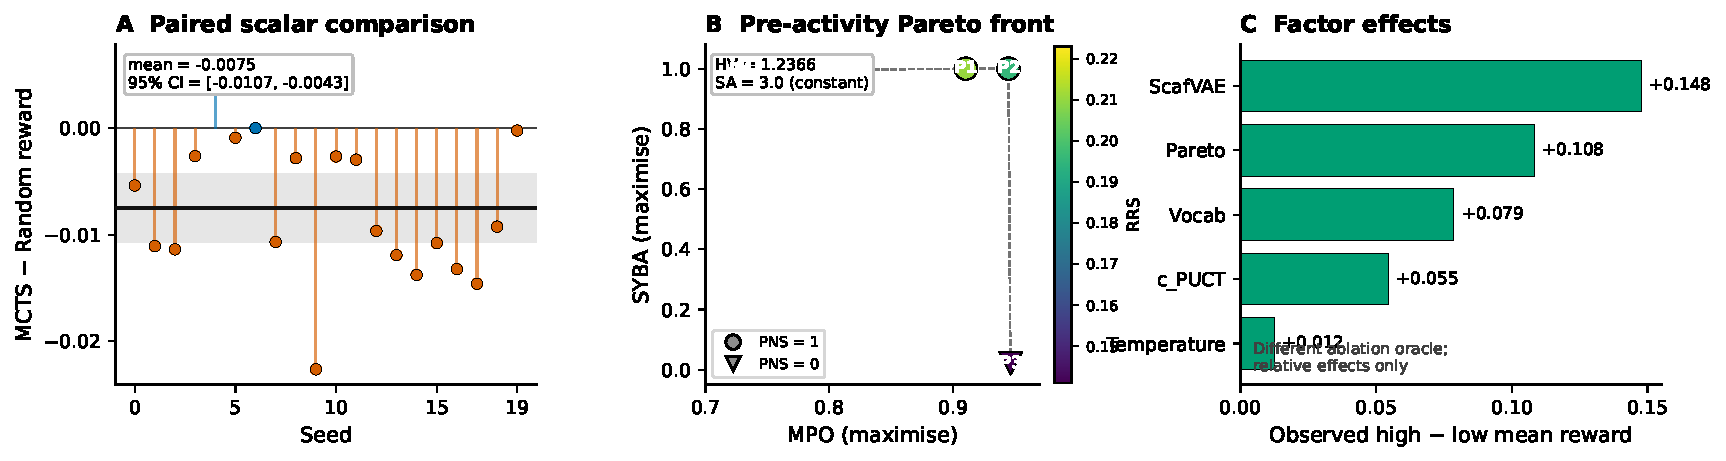
\includegraphics[width=0.98\textwidth]{Graphics/p4_evidence_overview.pdf}
  \caption{Integrated evidence overview generated directly from the deposited canonical data. (A) Paired per-seed differences between MCTS and random search under the v12 public-activity-augmented scalar reward; the horizontal band is the 95\% confidence interval for the mean difference. (B) The locked pre-activity Pareto front, with the RRS-informed proxy encoded by colour and the PNS-informed proxy by marker shape; SA is constant. (C) Observed high-minus-low main effects from the factorial ablation; these relative effects use a different oracle configuration and are not comparable to the main benchmark's absolute rewards.}
  \label{fig:overview}
\end{figure}

\begin{figure}[htbp]
  \centering
  
\includegraphics[width=0.72\textwidth]{Graphics/benchmark_efficiency.png}
  \caption{Computational efficiency of the four methods: best reward per seed versus wall-clock time (\Cref{tab:benchmark}). Error bars are one sample standard deviation. MCTS incurs the highest cost because the tree search evaluates the oracle at every construction step; greedy and the genetic algorithm are far cheaper.}
  \label{fig:efficiency}
\end{figure}

\subsection{Pareto front}
\label{sec:pareto_results}

We next analysed the deposited MCTS outputs under a pre-activity vector schema comprising MPO, SYBA, the RRS-informed chemotype proxy and the PNS-informed Tartarus docking proxy. The historical per-seed search records show that SYBA was constant at zero; the reported front is consequently a transparent post-hoc SYBA re-derivation from the discovered candidates, not evidence that the historical search optimised an informative SYBA signal. Across \num{20} independent seeds, the merged front contains four mutually non-dominated solutions with hypervolume \num{1.2366} (\Cref{fig:pareto}, \Cref{tab:pareto}).

\begin{figure}[htbp]
  \centering
  
\includegraphics[width=0.62\textwidth]{Graphics/pareto_front.png}
  \caption{Canonical \textbf{pre-activity} merged Pareto front from \num{20} independent Pareto-MCTS seeds. Marker shape encodes the PNS-informed Tartarus docking proxy; colour encodes the RRS-informed chemotype-similarity proxy. The four solutions are mutually non-dominated in the post-hoc re-derived schema of MPO, recomputed SYBA, the RRS-informed proxy and the PNS-informed proxy; SA is constant at \num{3.0} and excluded. Data: \texttt{results/pareto/merged\_pareto\_front.csv}.}
  \label{fig:pareto}
\end{figure}

\begin{figure}[htbp]
  \centering
  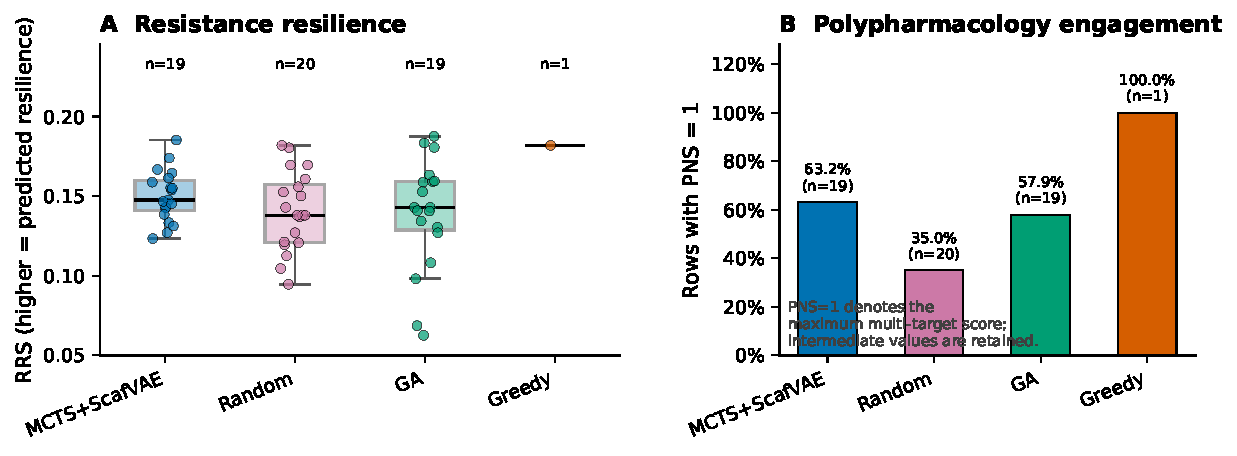
\includegraphics[width=0.86\textwidth]{Graphics/rrs_pns_profile.pdf}
  \caption{Domain-specific objective readout from the common pre-activity oracle applied to deposited best-in-seed molecules. (A) RRS distributions, with individual molecules shown and the valid row count reported for each method. (B) Fraction of valid rows with PNS = 1, the maximum value of the normalized three-column docking proxy; intermediate PNS values are retained in the source data. MCTS is shown descriptively against re-scored scalar baselines; the unequal counts and the single deterministic greedy row preclude an inferential method comparison. The canonical four-point MCTS front itself contains three PNS = 1 solutions and spans RRS = \num{0.141}--\num{0.223}.}
  \label{fig:rrs_pns}
\end{figure}

\begin{table}[htbp]
  \centering
  \caption{Canonical \textbf{pre-activity} merged Pareto front from \num{20} independent Pareto-MCTS seeds. All four points are mutually non-dominated in the post-hoc re-derived schema MPO, recomputed SYBA, RRS and PNS (SA is constant at \num{3.0} and excluded). SYBA was recomputed with the lich/conda classifier because the original run returned a constant fallback of zero; this table is not evidence of informative four-way optimisation during the historical search. SMILES and score tables are deposited.}
  \label{tab:pareto}
  \begin{tabular}{lccccc}
    \toprule
    Candidate & MPO $\uparrow$ & SYBA $\uparrow$ & SA$^{-1}$ $\uparrow$ & RRS & PNS \\
    \midrule
    P1 & \num{0.910} & \num{1.000} & \num{0.778} & \num{0.211} & \num{1.0} \\
    P2 & \num{0.945} & \num{1.000} & \num{0.778} & \num{0.196} & \num{1.0} \\
    P3 & \num{0.946} & \num{0.021} & \num{0.778} & \num{0.141} & \num{0.0} \\
    P4 & \num{0.729} & \num{0.994} & \num{0.778} & \num{0.223} & \num{1.0} \\
    \bottomrule
  \end{tabular}
\end{table}

P2 and P3 achieve the highest MPO values, yet P3 is synthetically inaccessible (SYBA $=\num{0.021}$). P1 and P4 remain highly accessible (SYBA $>\num{0.99}$) while trading potency. All four solutions share SA $= \num{3.0}$. Three of the four candidates also score PNS $=\num{1.0}$, the maximum value of the normalized three-column Tartarus docking proxy. This indicates a high value within the proxy panel, not simultaneous biological engagement of four Pf targets. Their RRS-informed proxy values span \num{0.141}--\num{0.223}, so the front includes both a higher-proxy/high-accessibility region and a high-potency/low-accessibility extreme. The re-scored baseline molecules provide an external context for this domain-specific readout: MCTS has mean RRS-informed proxy \num{0.150} across \num{19} valid rows and PNS $=1$ in \num{12}/\num{19} rows, compared with \num{0.141} and \num{7}/\num{20} for random search and \num{0.139} and \num{11}/\num{19} for GA (\Cref{fig:rrs_pns}). These are descriptive re-scoring results, not evidence of statistical superiority for MCTS on either proxy. The front nevertheless shows why retaining the domain-informed dimensions can be useful for audit and re-evaluation: it preserves a potency--accessibility trade-off while keeping resistance-related chemotype similarity and docking-proxy values visible in candidate provenance. Because SYBA was constant during the historical search, this dataset demonstrates transparent objective reconstruction more strongly than simultaneous optimisation of all four displayed dimensions. A high-MPO/low-SYBA extreme is thereby retained rather than silently removed by a single scalar objective. Quantitatively, over the space of all normalised scalar weights $w_{\text{MPO}}\in[0,1]$ on the normalised MPO--SYBA plane, P3 is selected by a fixed-weight scalar aggregation only for $w_{\text{MPO}}\gtrsim\num{0.997}$---a degenerate weighting (SYBA effectively ignored)---while P2 dominates the vast majority of the weight range (\Cref{tab:scalar_sweep}; full sweep deposited).

\begin{table}[htbp]
  \centering
  \caption{Agreement of fixed-weight scalar aggregation over the normalised MPO--SYBA plane: the weight interval $w_{\text{MPO}}$ over which each candidate is the scalar argmax, across all front and baseline molecules. P3 is selected only at a degenerate weight ($w_{\text{MPO}}\gtrsim\num{0.997}$). Data: \texttt{results/pareto/p4\_scalar\_weight\_sweep.csv}.}
  \label{tab:scalar_sweep}
  \begin{tabular}{lcS[table-format=1.3]}
    \toprule
    {Candidate / point} & {$w_{\text{MPO}}$ range} & {Fraction of $w$ space} \\
    \midrule
    P2 (high MPO \& SYBA) & $[0.0000,\ 0.9556]$ & \num{0.956} \\
    Baseline (mid)         & $[0.9556,\ 0.9968]$ & \num{0.041} \\
    P3 (high MPO, l.w SYBA) & $[0.9968,\ 1.0000]$ & \num{0.003} \\
    \bottomrule
  \end{tabular}
\end{table}

\subsection{Multi-objective front comparison against baselines}
\label{sec:front_comparison}

The scalar baselines were not optimised for the pre-activity vector objective. We therefore performed a transparent secondary analysis: each deposited per-seed best molecule was re-scored with the same MPO, SYBA, RRS-informed chemotype and PNS-informed docking proxies used for the canonical front, and a method-specific front was built under a common min--max normalisation (\Cref{tab:front_comp}). This is a re-scoring analysis, not a new benchmark, and SYBA was normalised with the same logistic transform used in the front recomputation ($1/(1+\exp(-s/5))$).

\begin{table}[htbp]
  \centering
  \caption{Multi-objective front comparison of the four generation methods. Each per-seed best molecule of the canonical \num{20}-seed benchmark was re-scored on the full objective (MPO, SYBA, RRS, PNS); the Pareto front of each method was then built and compared under a common min--max normalisation. Hypervolume and C-metric are the clean reference-independent metrics (C = fraction of the non-dominated union reference dominated by the method's front); IGD, IGD-${}_{\mathrm{loo}}$ (reference excluding the method's own points) and spread are reported for completeness. Data: \texttt{results/pareto/p4\_multiobj\_front\_summary.csv}.}
  \label{tab:front_comp}
  \begin{tabular}{llccccc}
    \toprule
    Method & Unique/20 & Front & HV & C-met. & IGD${}_{\mathrm{loo}}$ & Spread \\
    \midrule
    Random   & \num{20} & \num{8}  & \num{13.85} & \num{0.059} & \num{0.366} & \num{1.234} \\
    Greedy   & \num{1}  & \num{1}  & \num{16.59} & \num{0.765} & \num{0.416} & --- \\
    GA       & \num{19} & \num{8}  & \num{15.49} & \num{0.000} & \num{0.307} & \num{1.019} \\
    Baselines pooled & \num{40} & \num{11} & \num{15.52} & \num{0.000} & \num{0.307} & \num{0.903} \\
    \textbf{MCTS (front)} & \num{4} & \num{4} & \textbf{\num{18.99}} & \textbf{\num{0.824}} & \num{0.492} & \num{0.670} \\
    \bottomrule
  \end{tabular}
\end{table}

Two findings emerge. First, greedy search is \emph{deterministic} here: it returns the identical molecule across all \num{20} seeds, so its ``front'' reduces to a single point (unique count \num{1}). That single molecule is nonetheless strictly dominated by a point of the MCTS front (higher MPO \emph{and} higher RRS). The MCTS front attains the largest hypervolume (\num{18.99} under the common normalisation, above the \num{16.59} of the single greedy point, \num{15.52} of the pooled baseline front and \num{15.49} of GA) and the largest dominance coverage (C-metric \num{0.82}) of the non-dominated union reference. The IGD columns are shown for completeness but must be read with caution: with a leave-one-out reference (IGD${}_{\mathrm{loo}}$), the MCTS front is the most distant from the baseline-heavy reference, consistent with a designed front spanning the potency--accessibility trade-off rather than the broad baseline range. The hypervolume and C-metric, which are free of any comparison reference, are therefore the primary metrics reported here.

\subsection{Selection rule does not limit the front}
\label{sec:selection_ablation}

To test whether the gain of our framework arises from the \emph{selection} rule rather than the global Pareto stack, we ran an ablation in which tree selection is restricted, at each node, to the non-dominated children (a ParetoPUCT-style prior) before the PUCT score is applied. At equal budget (\num{700} iterations, \num{5} seeds), the two selection rules produce near-identical fronts (merged-front hypervolume under a common normalisation: scalar-proxy \num{15.56} vs Pareto-only \num{15.49}, $\Delta$ $\approx$ \num{0.5}\%). A paired per-seed sensitivity check quantifies what this study can and cannot establish: the per-seed hypervolume differences range from $\num{-1.78}$ to $+\num{1.81}$ (mean $+\num{0.53}$, paired $t=\num{0.85}$, $p>\num{0.05}$); with the observed between-seed deviation the minimal detectable effect is $\num{1.76}$ at \num{5} seeds and would remain $\num{0.88}$ even at \num{20} seeds (two-sided $\alpha=\num{0.05}$, power $=\num{0.8}$). Since the observed mean difference is smaller than this detectability floor, the near-null is not a power artefact that a larger run would overturn within a realistic budget; it is consistent with the scalar per-objective proxy not being a bottleneck. The value of Pareto-MCTS in the present design therefore comes from the global accumulation of a non-dominated front together with policy-guided exploration (both shared by both variants), rather than from the specific selection rule.

\subsection{Component and vocabulary ablations}
\label{sec:ablation}

A $2^{5}$ factorial experiment (ScafVAE policy, Pareto front, $c_{\text{PUCT}}$, temperature, vocabulary size; five replicates per cell) isolates the contribution of individual design choices. This ablation was retained from the pre-activity development protocol and uses a different oracle-weight configuration from v12; absolute rewards are therefore not comparable to the main benchmark, and only the within-ablation relative factor effects are interpreted (summarised in \Cref{fig:overview}).

The ScafVAE policy produces the largest gain ($\Delta = +\num{0.148}$), followed by the Pareto front ($\Delta = +\num{0.108}$) and the large vocabulary ($\Delta = +\num{0.079}$). Changing $c_{\text{PUCT}}$ from \num{2.0} to \num{1.0} improves reward by \num{0.055}; temperature has only a marginal effect.

A separate vocabulary ablation (all / medium / minimal / aromatic-only; \num{10} seeds each) yields a highly significant effect (one-way ANOVA $F=\num{350.1}$, $p=\num{1.12e-26}$). The aromatic-only vocabulary is significantly worse than the other three sets (Tukey HSD $p<\num{0.001}$), while the full and medium vocabularies do not differ significantly and the medium--minimal comparison is modest but significant ($p_{\mathrm{adj}}=\num{0.0052}$). Restricting the fragment set to aromatics alone therefore severely limits performance.

% ============================================================================
\section{Discussion}
% ============================================================================

\subsection{What the benchmark actually shows}

Within the curated medium fragment vocabulary and a fixed search budget, random search is a strong baseline and attains the highest mean scalar reward under both the baseline and the public-activity-augmented reward, as well as the single best seed. With its screened optimal configuration, MCTS trails by a modest margin on scalar reward (mean $\Delta = \num{-0.0075}$, $p = \num{0.000085}$; 95\% CI $[\num{-0.0107},\,\num{-0.0043}]$) and, under the multi-objective protocol, maintains and returns a Pareto front of non-dominated candidates. The practical value of the framework therefore lies not in peak single-objective performance but in the transparent exploration of trade-offs that scalar aggregation conceals.

This ranking is consistent with recent observations that simple baselines remain competitive in constrained fragment spaces~\citep{Jensen2019} and that the primary advantage of multi-objective MCTS is coverage of the non-dominated surface~\citep{Mothra2024}.

\subsection{Relation to prior multi-objective MCTS}

Mothra~\citep{Mothra2024} introduced a SMILES-based Pareto multi-objective MCTS and showed that Pareto fronts reveal trade-offs missed by scalar aggregation, and subsequent Pareto-MCTS generators have chiefly targeted protein--ligand binding~\citep{ParetoDrug2024} or dual-target scaffolds~\citep{CombiMOTS2026}. CombiMOTS~\citep{CombiMOTS2026} is itself malaria-motivated, framing dual-target engagement as a resistance-mitigation strategy, but its objectives remain binding/drug-likeness estimates rather than resistance or polypharmacology phenotypes. The contribution of the present work is a reproducible transfer to an antimalarial application domain with domain-informed objectives. We evaluate candidate generation jointly on potency (MPO), synthetic Bayesian accessibility (SYBA), an RRS-informed chemotype-similarity proxy and a PNS-informed Tartarus docking proxy, and pair this analysis with a scalar-reward benchmark against three baselines (random, greedy and genetic) across \num{20} independent seeds under a fixed search budget. The claim is deliberately bounded to this protocol and curated fragment space. Three implementation details are reported because they matter for reproducing the result: (i)~a scaffold-aware fragment policy replaces the uniform rollout prior, (ii)~dynamic progressive widening manages the large fragment branching factor, and (iii)~a rollout-degradation failure mode is diagnosed and corrected through global best-molecule tracking. The last point has the largest practical impact: without it, mean MCTS reward collapsed to approximately \num{0.24}; with it, reward rose by a factor of roughly \num{2.6}. The headline finding is intentionally honest: on the scalar reward, random search remains the strongest baseline, and the value of the Pareto-guided framework lies in the transparent coverage of multi-objective trade-offs rather than in a scalar superiority claim.

\subsection{Limitations}

Several limitations must be stated explicitly. First, the fragment vocabulary (approximately \num{108} fragments in the full set; medium subset used for the main benchmark) constrains accessible chemical space; results should not be extrapolated to open-ended SMILES generation. Second, molecular-diversity analysis is reported in the Supplementary Information in \Cref{SM-fig:sm_mds,SM-tab:sm_diversity}, where it is computed from the deposited best-in-seed molecule sets of the canonical benchmark; the main text emphasises the scalar ranking and the Pareto front, both fully deposited and reproducible. In particular, greedy search is deterministic here---it returns the identical molecule across all \num{20} seeds---so its deposited set is a single point rather than a diverse panel. Third, SYBA scores on the Pareto front were recomputed post-hoc after the original search returned a constant zero fallback; the recomputation, the resulting front and the verification scripts are documented and deposited. Fourth, activity, resistance-resilience and polypharmacology labels remain computational proxies; prospective experimental validation is required. In particular, the present fragment space produces a narrow RRS range and predominantly discrete PNS values, so the study demonstrates objective integration and candidate-selection provenance more strongly than it demonstrates broad phenotypic separation. Finally, MCTS cross-seed variability is modest in the canonical scalar benchmark ($\mathrm{SD}=\num{0.0068}$), but this does not establish robustness outside the curated fragment vocabulary or the fixed budget. The deposited per-seed outputs make that uncertainty inspectable.

\subsection{Implications for antimalarial design}

A distinctive feature of the present setup is that domain-informed proxy signals are recorded alongside candidate retention rather than appearing only in an opaque final ranking. Whereas prior Pareto-MCTS generators commonly optimise binding, drug-likeness, toxicity or dual-target objectives~\citep{Mothra2024,ParetoDrug2024,CombiMOTS2026}, this implementation adds an RRS-informed chemotype-similarity proxy and a PNS-informed Tartarus docking proxy alongside potency and accessibility. The historical run exposes the resistance-related and docking-derived proxy signals during generation, while SYBA is explicitly limited to post-hoc re-evaluation because its search-time fallback was constant. The current data also define the limit of that claim: the RRS-informed proxy spans only \num{0.141}--\num{0.223}, and PNS equals \num{1.0} for three of four front points. The present study consequently demonstrates auditable objective integration and Pareto retention, not broad biological discrimination or direct resistance validation.

% ============================================================================
\section{Methods}
% ============================================================================

\subsection{Molecular environment}
\label{sec:env}

De novo generation is formulated as a Markov decision process. The state is a partially constructed molecule (canonical SMILES); actions append one fragment from a curated vocabulary at a regiospecific attachment point. Episode termination occurs after at most \num{10} construction steps or upon violation of a reactivity filter. The main benchmark uses the medium fragment subset; ablations also evaluate the full, minimal and aromatic-only vocabularies.

\subsection{MCTS with scaffold-aware policy}
\label{sec:mcts}

The agent follows the standard four-phase MCTS loop (selection, expansion, rollout, backpropagation) rooted at benzene, with $N_{\text{iter}}=\num{1000}$. Selection maximises the PUCT score
\begin{equation}
  a^{*} = \arg\max_{a}\;
  \frac{Q(s,a)}{N(s,a)}
  + c_{\text{PUCT}}\,P(a\mid s)\,\frac{\sqrt{N(s)}}{1+N(s,a)},
\end{equation}
with $c_{\text{PUCT}}=\num{5.0}$. The policy $P(a\mid s)$ combines ChEMBL27 fragment frequencies, scaffold Tanimoto compatibility and a reactivity penalty via a softmax. Dynamic progressive widening limits the number of expanded actions at each node to $\max(5,\,k\,N^{\alpha})$ with $k=\num{1.0}$ and $\alpha=\num{0.5}$. A virtual-loss term ($\nu=\num{0.01}$) discourages repeated selection of the same child within a single search.

\subsection{Global best-molecule tracking}
\label{sec:rollout_fix}

Policy-biased rollouts can degrade a high-quality intermediate by subsequent fragment additions. During each rollout the oracle is therefore evaluated at every construction step; the highest-scoring intermediate---rather than the terminal state---is returned. This change recovered a factor of approximately \num{2.6} in mean reward relative to the uncorrected agent.

\subsection{Pareto front maintenance}
\label{sec:pareto}

The agent maintains a global non-dominated \textbf{pre-activity} candidate pool over the recorded objective schema
\[
\mathbf{f}(s)=\bigl(f_{\text{MPO}}(s),\,f_{\text{SYBA}}(s),\,f_{\text{RRS}}(s),\,f_{\text{PNS}}(s)\bigr),
\]
with minimisation objectives converted to maximisation by negation. In the historical run, SYBA was constant at zero in every per-seed record and was automatically excluded as a non-informative dimension during search; SA was likewise constant ($\mathrm{SA}=\num{3.0}$) and excluded. The final four-point front was re-derived after SYBA recomputation, so its displayed four-dimensional non-dominance is a post-hoc audited result, not a claim of four-way informative optimisation during the original search. After each rollout the best intermediate molecule is tested for dominance; dominated members are removed. The hypervolume indicator is computed with the active (non-constant) objectives only: each active objective is min--max normalised to $[0,1]$, and the hypervolume is evaluated with respect to a reference point $\mathbf{r}=\num{1.1}$ (slightly worse than the worst normalised value of $1$) in each active dimension, so that the reported value lies in $[0,1.1]^{k}$ for $k$ active objectives. For PUCT selection a scalar proxy $Q(s,a)$ is obtained by summing the min--max normalised components that vary in the run; the full vector is stored for candidate-pool updates and post-hoc analysis. In the historical run, the constant SYBA fallback contributed no information to $Q(s,a)$. This distinction matters here because SYBA was constant during the historical search and contributed no information to $Q(s,a)$.

\subsection{Scoring oracles}
\label{sec:oracles}

Each molecule is scored by an aggregator returning MPO, SYBA, SA, docking-derived terms, an RRS-informed chemotype-similarity proxy, a PNS-informed normalized Tartarus docking proxy, and public-activity proximity (activity). The historical pre-activity CSVs must be read with the SYBA provenance caveat below: their SYBA field is a constant fallback, not an informative search-time measurement. RRS uses Morgan/Tanimoto similarity to P2 reference chemotypes; the current implementation does not propagate per-target WT/mutant ratios. PNS averages the detected Tartarus columns \texttt{score\_1syh}, \texttt{score\_6y2f} and \texttt{score\_4lde}; it is not a direct PfDHFR/PfCRT/PfATP4/PfClpP panel. These proxies remain displayed dimensions of the post-hoc audited pre-activity front, but their biological validation is outside the present P4 run. The RRS-informed and PNS-informed proxy signals were available during historical candidate discovery; the constant SYBA fallback was not informative during that run. In the v12 scalar benchmark, RRS and PNS are disabled and are not silently substituted for the public-activity term. Default scalar-reward weights are $w_{\text{MPO}}=\num{0.27}$, $w_{\text{docking}}=\num{0.225}$, $w_{\text{SYBA}}=\num{0.135}$, $w_{\text{SA}}=\num{0.045}$, $w_{\text{RRS}}=\num{0.135}$, $w_{\text{PNS}}=\num{0.09}$, $w_{\text{activity}}=\num{0.10}$. The activity oracle scores a molecule by its maximum Morgan-2 Tanimoto to the \num{19321} experimentally active antimalarial compounds of the independent public ChEMBL IC50/EC50 dataset (\num{22447} molecules), scaled continuously (Tanimoto $\le \num{0.20}$ gives a soft gradient; $\num{0.20}$--$\num{1.0}$ maps linearly). The four-method v12 scalar benchmark uses the reduced reward \texttt{compute\_mpo\_reward} with weights $w_{\text{MPO}}=\num{0.36}$, $w_{\text{docking}}=\num{0.315}$, $w_{\text{SYBA}}=\num{0.135}$, $w_{\text{SA}}=\num{0.09}$ and $w_{\text{activity}}=\num{0.10}$; RRS and PNS are disabled in this benchmark because they require external P2 mutant and network data. Separately, the canonical Pareto-MCTS front reported in \Cref{tab:pareto} was generated under the pre-activity vector objective set (MPO, SYBA, RRS, PNS), with activity excluded from its dominance check and hypervolume. Thus, the v12 activity term changes only the scalar benchmark and does not retroactively alter the locked Pareto front. MPO and docking scores are drawn from precomputed libraries where available; QED serves as an MPO fallback for novel structures. SYBA on the reported Pareto front was recomputed with the lich/conda classifier after the original run returned a constant zero fallback. The historical search-time SYBA fallback is not interpreted as a validated accessibility measurement. The accessibility column reported in \Cref{tab:pareto} is the linear transform $\mathrm{SA}^{-1} = (10 - \mathrm{SA})/9$ of the raw Ertl score, so that the shared raw value $\mathrm{SA} = \num{3.0}$ corresponds to $\mathrm{SA}^{-1} = \num{0.778}$; the deposited CSV stores the raw value.

\subsection{Statistical analysis and reproducibility}

All searches are seeded; the specific seed integers and the random-number generators (NumPy \texttt{default\_rng}, seeded per method and per seed with no cross-method state leakage) are fixed in the committed script. The four-method benchmark uses \num{20} independent seeds; ablations use five or ten replicates as indicated. Paired $t$-tests are reported for the two planned head-to-head comparisons (MCTS--random and MCTS--GA); because both are pre-specified primary comparisons, we report unadjusted two-sided $p$-values and note that both remain significant after a conservative Bonferroni adjustment across the two primaries (adjusted threshold $\num{0.025}$): MCTS--random $p = \num{0.000085}$, MCTS--GA $p<\num{0.0001}$. The vocabulary ablation is tested with a one-way ANOVA (three degrees of freedom between groups) followed by pairwise Tukey HSD post-hoc comparisons. The benchmark was re-run for this submission with the committed script \texttt{p4\_mcts\_benchmark.py} and a value-preserving vectorisation of the docking Tanimoto scan (verified identical on held-out molecules); all \num{20} per-seed runs reproduce deterministically from the deposited code and data, and the best-in-seed molecule sets are deposited alongside the scalar rewards. Analyses were executed with Python 3.11, RDKit, NumPy, SciPy and pymoo; exact dependency versions are recorded in the repository environment file. Code, configuration files, molecule lists and score tables are released under the MIT licence in the public repository \url{https://github.com/NanaEngo/Malaria_codesV2}. The Zenodo DOI \url{https://doi.org/10.5281/zenodo.19608875} is reserved, but the upload remains pending.

% ============================================================================
\section{Conclusions}
% ============================================================================

A Pareto-guided MCTS agent equipped with a scaffold-aware fragment policy trails random search by a modest margin on the v12 scalar reward (mean $\Delta = \num{-0.0075}$, $p = \num{0.000085}$, 95\% CI $[\num{-0.0107},\,\num{-0.0043}]$ at the screened optimal configuration). In the separate historical pre-activity analysis, it yields an audited front of non-dominated candidates; the RRS-informed and PNS-informed proxies were available during candidate discovery, whereas SYBA was recomputed post hoc. The factorial ablation identifies large effects for the policy and Pareto components, although its oracle configuration differs from v12. Within the studied fragment space, random search remains a strong scalar baseline; the added value of MCTS is transparent objective-space exploration, not scalar superiority or direct biological validation. The code and currently released data needed for reproduction are available in the public repository; the reserved Zenodo deposit remains pending.

% ============================================================================
\section*{List of Abbreviations}
% ============================================================================

\textbf{MCTS:} Monte Carlo tree search; \textbf{MPO:} multi-parameter optimisation; \textbf{SYBA:} synthetic Bayesian accessibility; \textbf{SA:} synthetic accessibility score; \textbf{RRS:} resistance resilience score; \textbf{PNS:} polypharmacology-network score; \textbf{GA:} genetic algorithm; \textbf{PUCT:} polynomial upper confidence trees; \textbf{SMILES:} simplified molecular-input line-entry system; \textbf{ChEMBL:} ChEMBL bioactivity database; \textbf{PF-MPO:} parallel fragment multi-objective; \textbf{FCD:} Fr\'echet ChemNet distance; \textbf{HV:} hypervolume; \textbf{MDS:} multidimensional scaling; \textbf{CI:} confidence interval.

% ============================================================================
\section*{Data availability}
% ============================================================================

All data supporting the conclusions are released under the MIT licence in the public repository \url{https://github.com/NanaEngo/Malaria_codesV2}, which is immediately available to reviewers. The Zenodo DOI \url{https://doi.org/10.5281/zenodo.19608875} is reserved; the upload is pending and is not yet an existing archive. The deposit includes: (i)~the canonical 20-seed four-method benchmark tables and best-in-seed SMILES (\texttt{results/benchmark\_molecules\_opt/} for the baseline reward and \texttt{results/benchmark\_molecules\_opt\_v12/} for the public-activity-augmented reward); (ii)~per-seed and merged Pareto fronts with the post-hoc SYBA recomputation log (\texttt{results/pareto/}); (iii)~diversity metrics and MDS coordinates (\texttt{results/diversity/}); (iv)~component and vocabulary ablation summaries; and (v)~analysis and provenance-check scripts.

\section*{Competing interests}
The authors declare that they have no competing interests.

\section*{Authors' contributions}
MVST: conceptualization, methodology, software, formal analysis, writing---original draft. JPTN: methodology, supervision, writing---review \& editing. PS: data curation, writing---review \& editing. WFM: validation, writing---review \& editing. SGNE: supervision, writing---review \& editing. All authors read and approved the final manuscript.

\section*{Acknowledgements}
We thank the developers of RDKit, SYBA and the open-source MCTS literature for foundational tools and ideas. Computational resources were provided by the University of Yaound\'{e} I HPC facility.

\section*{Funding}
This research received no specific external funding. Computational resources were provided by the University of Yaound\'{e} I HPC facility.

\section*{Ethics approval and consent to participate}
Not applicable.

\section*{Consent for publication}
Not applicable.

\section*{Use of Artificial Intelligence}
During the preparation of this work the authors used AI assistants to support code development and data analysis scripting. The authors reviewed and edited all AI-assisted output and take full responsibility for the content of this article. No generative AI tool is listed as an author. All computational results, statistical analyses, and quantitative claims were generated, verified, and deposited by the authors.

% ============================================================================
\bibliographystyle{unsrtnat}
\bibliography{P4_Bibliography}

\end{document}
